%% Ejemplo de la plantilla de latex para las diapositivas del Máster en IA 

%%%%%%%%%%%%%%%%%%%%%%%%%%%%
%% Valores para el ratio de aspecto: 43, 169 
\documentclass[10pt, envcountsect, presentation, aspectratio=169]{beamer}
%%%%%%%%%%%%%%%%%%%%%%%%%%%%

%%%%%%%%%%%%%%%%%%%%%%%%%%%%
%% Incluir fichero de estilo del máster
\input plantillaTAREA.sty
%%%%%%%%%%%%%%%%%%%%%%%%%%%%

\let\Tiny=\tiny
%\usepackage[latin1]{inputenc}
\usepackage[utf8]{inputenc}
\usepackage[spanish]{babel}
\usepackage{pgf}
\usepackage{latexsym}
\usepackage{amssymb,amsmath}
\usepackage{xspace}
\usepackage[olditem,oldenum]{paralist}
\usepackage{tikz}
\usetikzlibrary{snakes,arrows,shapes}
\usetikzlibrary{positioning}
\usetikzlibrary{arrows,automata}
\usepackage[T1]{fontenc}
\usepackage{psfrag}
\usepackage{multirow}
\usepackage{xmpmulti}
\usepackage[absolute, overlay]{textpos}
\usepackage{pgfpages}
\usepackage{pgf}
\usepackage{colortbl}
\usepackage{xcolor}
\usepackage{color}

%%%%%%%%%%%%%%%%%%%%%%%%%%%%
%% Información que aparecerá en la portada
\title[Nombre]{Modelos de Computación}
\subtitle{Entrega de Lenguajes y Computabilidad} % short title for footer

\author[Carrillo G., Gallego J., Ibarrola Y.] % Para el pie de página, poner los autores abreviados separados por comas.
{
	\sc{Ginés Carrillo Ibáñez}\\  % Autor 1
	\textit{Grupo 1.Subgrupo 9}\\
	\sc{Juan Diego Gallego Nicolás}\\ % Autor 2
	\textit{Grupo 1.Subgrupo 9}\\ 
	\sc{Juan Diego Gallego Nicolás}\\ % Autor 3
	\textit{Grupo 1. Subgrupo 9}\\ 
}

\institute[GII]% % Poner las iniciales de los diferentes departamentos de los autores separadas por comas.
{
	\textit{Universidad de Murcia}
}

\date{2024/2025} % Curso académico

%%%%%%%%%%%%%%%%%%%%%%%%%%%%%%%%%%
%% Contenido de las diapositivas
\setbeamerfont{normal text}{size=\normalsize} % Modifica el tamaño del texto de las diapositivas.
\AtBeginDocument{\usebeamerfont{normal text}}

%%%%%%%%%%%%%%%%%%%%%%%%%%%%%%%%%%

\newcommand{\ldfa}{\ensuremath{\mathcal L_{DFA}}}
\newcommand{\lnfa}{\ensuremath{\mathcal L_{NFA}}}
\newcommand{\ler}{\ensuremath{\mathcal L_{ER}}}
\newcommand{\lreg}{\ensuremath{\mathcal {REG}}}
\newcommand{\lcf}{\ensuremath{\mathcal CF}}
\newcommand{\lpda}{\ensuremath{\mathcal L_{PDA}}}
\newcommand{\lpdav}{\ensuremath{\mathcal L_{PDA^v}}}
\newcommand{\lpdad}{\ensuremath{\mathcal L_{PDAD}}}
\newcommand{\lgr}{\ensuremath{\mathcal L_{GCF}}}
\newcommand{\ld}{\ensuremath{\mathcal {DEC}}}
\newcommand{\lr}{\ensuremath{\mathcal {RE}}}
\newcommand{\halt}{\ensuremath{\mathsf{HALT}}}
\newcommand{\fon}{\ensuremath{FO(\mathbb N)}}
\newcommand{\pol}{\ensuremath{\mathcal P}}
\newcommand{\npol}{\ensuremath{\mathcal{NP}}}
\newcommand{\cnpol}{\ensuremath{\mathcal{CO-NP}}}
\newcommand{\cnlo}{\ensuremath{\mathcal{CO-NLOG}}}
\newcommand{\cnpols}{\ensuremath{\mathcal{CO-NPSPACE}}}
\newcommand{\fo}{\ensuremath{FO}}
\newcommand{\lop}{\ensuremath{LP}}
\newcommand{\cnf}{\ensuremath{_{cnf}}}
\newcommand{\tcnf}{\ensuremath{_{3cnf}}}
%\newcommand{\cnf}{\ensuremath{LP_{cnf}}}
%\newcommand{\tcnf}{\ensuremath{LP_{3cnf}}}
\newcommand{\qlop}{\ensuremath{QLP}}
\newcommand{\dcnf}{\ensuremath{LP_{2cnf}}}
\newcommand{\pols}{\ensuremath{\mathcal{PSPACE}}}
\newcommand{\npols}{\ensuremath{\mathcal{NPSPACE}}}
\newcommand{\lo}{\ensuremath{\mathcal{LOG}}}
\newcommand{\nlo}{\ensuremath{\mathcal{NLOG}}}
\newcommand{\ext}{\ensuremath{\mathcal{EXPTIME}}}
\newcommand{\extn}{\ensuremath{\mathcal{NEXPTIME}}}
\newcommand{\exts}{\ensuremath{\mathcal{EXPSPACE}}}
\newcommand{\ej}{{\color{green}ejemplo}}
\newcommand{\usigma}{\ensuremath{\mathcal U}_{\Sigma}}
\newcommand{\mt}{\ensuremath{\mathcal {MT}}} 
\newcommand{\pnp}{¿\ensuremath{\mathcal{P}=\mathcal{NP}}? }

%%%%%%%%%%%%%%%%%%%%%%%%%%%%%%%%%%

\begin{document}	

%%%%%%%%%%%%%%%%%%%%%%%%%%%%%%%%%%

%%%%%%%%%%%%%%%%%%%%%%%%%%%%%%%%%%

\begin{frame}[plain]
	\titlepage
\end{frame}

%%%%%%%%%%%%%%%%%%%%%%%%%%%%%%%%%%

\begin{frame}{Sección Cuarto de Punto}{Ejercicio 0}
% \vskip -1cm % Para subir (-) o bajar el texto
\textbf{Título de la subsección (o del concepto en su caso)}
	\begin{itemize}
	\item Texto ...
	\item Texto ... \citep{Russell2020} ...
		\begin{itemize}
		\normalsize % Quítalo si quieres que se reduzca automáticamente el tamaño del texto	
		\item[--] Texto ...
		
			\begin{itemize}
			\normalsize % Quítalo si quieres que se reduzca automáticamente el tamaño del texto
			\item[$\bullet$] Texto ...
			\end{itemize}	
			\end{itemize} 
	\item Texto ...		
	\item Texto ...
	\end{itemize}
\end{frame}

%%%%%%%%%%%%%%%%%%%%%%%%%%%%%%%%%%

\begin{frame}{Sección Cuarto de Punto}{Ejercicio 1}
    % \vskip -1cm % Para subir (-) o bajar el texto
    \textbf{Enunciado}
    \begin{itemize}
        \item Con los modelos de computación  siguientes,  escribe una lista  ordenada en modo ascendente según su capacidad expresiva. Entre un modelo y el siguiente establece  la relación  ($\equiv$) o ($\prec$) o  según corresponda.
		\begin{enumerate}[I)]
            \item El $\lambda-$Cálculo
            \item El modelo dado por $(Q,\Sigma,\Gamma,\delta,A_0,q_0,F)$, donde  $Q$ es un conjunto finito de estados, $\Sigma$ y $\Gamma$ son alfabetos, $\delta:Q\times \Sigma_\epsilon\times\Gamma_\epsilon\rightarrow 2^{(Q\times\Gamma_\epsilon)}$ es  una función de transición, $A_0$ es el símbolo inicial de la pila, y $q_0\in Q$ es el estado inicial. 
            \item El modelo dado por $(Q,\Sigma,\Gamma,\delta,A_0,q_0,q_f)$, donde  $Q$ es un conjunto finito de estados, $\Sigma$ y $\Gamma$ son alfabetos, $\Sigma_\epsilon=\Sigma \cup \{\epsilon\}$, $\Gamma_\epsilon=\Gamma \cup \{\epsilon\}$, $\delta:Q\times \Sigma_\epsilon\times\Gamma_\epsilon\rightarrow 2^{(Q\times\Gamma_\epsilon)}$ es  una  función de transición, $A_0$ es el símbolo inicial de la pila, y $q_0\in Q$ es el estado inicial. 
            \item ...
        \end{enumerate}
	\end{itemize}
\end{frame}

%%%%%%%%%%%%%%%%%%%%%%%%%%%%%%%%%%

\begin{frame}{Sección Cuarto de Punto}{Ejercicio 1}
    \textbf{Solución}\\
    \begin{itemize}
        \item $\mathcal{AFD}$
    \end{itemize}
\end{frame}

%%%%%%%%%%%%%%%%%%%%%%%%%%%%%%%%%%

\begin{frame}{Sección Cuarto de Punto}{Ejercicio 1}
    \textbf{Solución}\\
    \begin{itemize}
        \item $\mathcal{DFA} \equiv \mathcal{NDFA}$
        \item[X)] El modelo dado por  $(Q,\Sigma_\epsilon,\delta,q_0,F)$, donde  $Q$ es un   conjunto finito de estados, $\Sigma$ es un alfabeto, $\Sigma_\epsilon=\Sigma \cup \{\epsilon\}$, $\delta:Q\times \Sigma_\epsilon\rightarrow 2^{Q}$ es una función de transición, $q_0\in Q$ es el  estado inicial, y $F\subseteq Q$ es el conjunto de estados finales.
    \end{itemize}
\end{frame}

%%%%%%%%%%%%%%%%%%%%%%%%%%%%%%%%%%

\begin{frame}{Sección Cuarto de Punto}{Ejercicio 1}
    \textbf{Solución}\\
    \begin{itemize}
        \item $\mathcal{DFA} \equiv \mathcal{NDFA} \prec \mathcal{DPDA}$
        \item[VI)] El modelo dado por $(Q,\Sigma,\Gamma,\delta,A_0,q_0,F)$, donde  $Q$ es un conjunto finito de estados, $\Sigma$ y $\Gamma$ son alfabetos, $\delta:Q\times \Sigma_\epsilon\times\Gamma_\epsilon\rightarrow(Q\times\Gamma_\epsilon)$ es  una función de transición, que cumple que para cada $q \in Q$, cada $a \in \Sigma$ y cada $x \in \Gamma$, exactamente una de estas reglas de transición $\delta(q,a,x),\delta(q,a,\epsilon),\delta(q,\epsilon,x),\delta(q,\epsilon,\epsilon)$ es distinta de  $\emptyset$; $A_0$ es el símbolo inicial de la pila, $q_0\in Q$ es el estado inicial, y $F\subseteq Q$ es el conjunto de  estados finales.
    \end{itemize}
\end{frame}

%%%%%%%%%%%%%%%%%%%%%%%%%%%%%%%%%%

\begin{frame}{Sección Cuarto de Punto}{Ejercicio 1}
    \textbf{Solución}\\
    \begin{itemize}
        \item $\mathcal{DFA} \equiv \mathcal{NDFA} \prec \mathcal{DPDA} \prec \mathcal{PDA}$
        \item[II)] El modelo dado por $(Q,\Sigma,\Gamma,\delta,A_0,q_0,F)$, donde  $Q$ es un conjunto finito de estados,  $\Sigma$ y $\Gamma$ son alfabetos, $\delta:Q\times \Sigma_\epsilon\times\Gamma_\epsilon\rightarrow 2^{(Q\times\Gamma_\epsilon)}$ es  una función de transición, $A_0$ es el símbolo inicial de la pila, y $q_0\in Q$ es el estado inicial. 
    \end{itemize}
\end{frame}

%%%%%%%%%%%%%%%%%%%%%%%%%%%%%%%%%%

\begin{frame}{Sección Cuarto de Punto}{Ejercicio 1}
    \textbf{Solución}\\
    \begin{itemize}
        \item $\mathcal{DFA} \equiv \mathcal{NDFA} \prec \mathcal{DPDA} \prec \mathcal{PDA} \equiv \mathcal{PDA}^v$
        \item[III)] El modelo dado por $(Q,\Sigma,\Gamma,\delta,A_0,q_0,q_f)$, donde  $Q$ es un conjunto finito de estados, $\Sigma$ y $\Gamma$ son alfabetos, $\Sigma_\epsilon=\Sigma \cup \{\epsilon\}$, $\Gamma_\epsilon=\Gamma \cup \{\epsilon\}$, $\delta:Q\times \Sigma_\epsilon\times\Gamma_\epsilon\rightarrow 2^{(Q\times\Gamma_\epsilon)}$ es  una  función de transición, $A_0$ es el símbolo inicial de la pila, y $q_0\in Q$ es el estado inicial.         
    \end{itemize}
\end{frame}

%%%%%%%%%%%%%%%%%%%%%%%%%%%%%%%%%%

\begin{frame}{Sección Cuarto de Punto}{Ejercicio 1}
    \textbf{Solución}\\
    \begin{itemize}
        \item $\mathcal{DFA} \equiv \mathcal{NDFA} \prec \mathcal{DPDA} \prec \mathcal{PDA} \equiv \mathcal{PDA}^v \prec \mathcal{STM}$
        \item[VII)] El modelo dado por $(Q,\Sigma,\Gamma,\delta,q_0,q_f)$, donde $Q$ es un conjunto finito de estados, $\Sigma$ y $\Gamma$ son alfabetos de modo que $B\in\Gamma$,  $\Sigma\subseteq\Gamma$ y $B \notin \Sigma$, $\delta:Q\times\Gamma\rightarrow 2^{Q\times\Gamma\times\{L,R, S\}}$ es  una función de transición, $q_0\in Q$ es el estado inicial, y $q_f\in Q$ es el estado final.     
    \end{itemize}
\end{frame}

%%%%%%%%%%%%%%%%%%%%%%%%%%%%%%%%%%

\begin{frame}{Sección Cuarto de Punto}{Ejercicio 1}
    \textbf{Solución}\\
    \begin{itemize}
        \item $\mathcal{DFA} \equiv \mathcal{NDFA} \prec \mathcal{DPDA} \prec \mathcal{PDA} \equiv \mathcal{PDA}^v \prec \mathcal{STM} \equiv k-\mathcal{TM}$
        \item[IX)] El modelo dado por $(Q,\Sigma,\Gamma,\delta,q_0,q_f)$, donde $Q$ es un conjunto finito de estados, $\Sigma$ y $\Gamma$ son alfabetos de modo que $B\in\Gamma$,  $\Sigma\subseteq\Gamma$ y $B \notin \Sigma$, $q_0\in Q$ es el estado inicial, y $q_f\in Q$ es el estado final y la función de transición es:
        \begin{small}
            $\delta:Q\times\underbrace{\Gamma\times\ldots\times\Gamma}_k\rightarrow Q\times\underbrace{\Gamma\times\{L,R,S\}\times\ldots\times\Gamma\times\{L,R,S\}}_k$.
        \end{small} 
    \end{itemize}
\end{frame}

%%%%%%%%%%%%%%%%%%%%%%%%%%%%%%%%%%

\begin{frame}{Sección Cuarto de Punto}{Ejercicio 1}
    \textbf{Solución}\\
    \begin{itemize}
        \item $\mathcal{DFA} \equiv \mathcal{NDFA} \prec \mathcal{DPDA} \prec \mathcal{PDA} \equiv \mathcal{PDA}^v \prec \mathcal{STM} \equiv k-\mathcal{TM} \equiv TCL$
        \item[I)] El $\lambda-$Cálculo.
        \item[IV)] Máquina de Turing con cinta finita a la izquierda e infinita a la derecha, que sólo tiene movimiento hacia la derecha y un movimiento que retorna el cabezal de lectura/escritura a la celdilla más a la izquierda.
        \item[V)] El lenguaje de programación Python
        \item[VIII)] Un lenguaje de programación Turing-completo 
    \end{itemize}
\end{frame}

%%%%%%%%%%%%%%%%%%%%%%%%%%%%%%%%%%

\begin{frame}{Sección Cuarto de Punto}{Ejercicio 2}
% \vskip -1cm % Para subir (-) o bajar el texto
\textbf{Enunciado}
	\begin{itemize}
        \item Agrupa juntas las siguientes definiciones equivalentes:
        \begin{enumerate}[1.]
            \item $\mathcal{P}( \Sigma ^ *)$
            \item Conjunto de los lenguajes regulares
            \item Conjunto de los problemas de decisión computables
            \item $\lpdav$
            \item Conjunto de los lenguajes altamente indecidibles
            \item ...
        \end{enumerate}
	\end{itemize}
\end{frame}

%%%%%%%%%%%%%%%%%%%%%%%%%%%%%%%%%%

\begin{frame}{Sección Cuarto de Punto}{Ejercicio 2}
    \textbf{Solución}\\
    \begin{itemize}
        \item $\lreg$
        \item[2.] Conjunto de los lenguajes regulares
        \item[15.] $\ldfa$
        \item[16.] Clase en la que se situaría todo lenguaje $L$ que cumple que $|L|$ es finito
        \item[20.] $\lnfa$
        \item[21.] Conjunto de lenguajes reconocibles por DFAs
        \item[22.] Conjunto de los lenguajes que se pueden describir mediante expresiones regulares
        \item[24.] Conjunto de lenguajes reconocibles por NDFAs
    \end{itemize}
\end{frame}

%%%%%%%%%%%%%%%%%%%%%%%%%%%%%%%%%%

\begin{frame}{Sección Cuarto de Punto}{Ejercicio 2}
    \textbf{Solución}\\
    \begin{itemize}
        \item $\lpdad$
        \item[19.] Conjunto de lenguajes reconocibles por PDAs deterministas por estado final
    \end{itemize}
\end{frame}

%%%%%%%%%%%%%%%%%%%%%%%%%%%%%%%%%%

\begin{frame}{Sección Cuarto de Punto}{Ejercicio 2}
    \textbf{Solución}\\
    \begin{itemize}
        \item $\lcf$
        \item[4.] $\lpdav$ 
        \item[8.] Conjunto de lenguajes reconocibles por PDAs no deterministas por pila vacía
        \item[11.] Conjunto de los lenguajes generables por gramáticas libres de contexto
        \item[17.] $\lpda$
        \item[18.] $\lgr$
    \end{itemize}
\end{frame}

%%%%%%%%%%%%%%%%%%%%%%%%%%%%%%%%%%

\begin{frame}{Sección Cuarto de Punto}{Ejercicio 2}
    \textbf{Solución}\\
    \begin{itemize}
        \item $\ld$
        \item[3.] Conjunto de los problemas de decisión computables
        \item[12.] Conjunto de los lenguajes para los que existe una MT determinista de dos cintas que los decide
        \item[23.] Clase formada por todo lenguaje L que cumple que tanto él como su complementario tienen máquinas de turing que los enumeran
        \item[30.] Conjunto formado por todo lenguaje L para el que se puede construir un algoritmo en python capaz de aceptar las palabras que pertenecen a L y de rechazar las que no pertenecen a L
    \end{itemize}
\end{frame}

%%%%%%%%%%%%%%%%%%%%%%%%%%%%%%%%%%

\begin{frame}{Sección Cuarto de Punto}{Ejercicio 2}
    \textbf{Solución}\\
    \begin{itemize}
        \item $\lr$
        \item[6.] Conjunto de los lenguajes Turing-reconocibles
        \item[9.] Conjunto de los lenguajes recursivamente enumerables
        \item[13.] Conjunto de lenguajes para los que se puede construir un algoritmo en java capaz de reconocer las palabras que pertenecen al lenguaje
        \item[14.] Conjunto de lenguajes semidecidibles
    \end{itemize}
\end{frame}

%%%%%%%%%%%%%%%%%%%%%%%%%%%%%%%%%%

\begin{frame}{Sección Cuarto de Punto}{Ejercicio 2}
    \textbf{Solución}\\
    \begin{itemize}
        \item $\mathcal{CO-RE}$
        \item[10.] Conjunto de los lenguajes cuyos complementarios son Turing-reconocibles 
        \item[25.] Clase formada por todo lenguaje $L$ para el que existe una K-MT que es capaz de acteptar todas las palabras fuera de $L$ y de no aceptar todas las que están dentro de $L$
        \item[28.] Clase en la que se situaría un lenguaje $L$ para el que tenemos una MT que acepta todas y sólo aquellas cadenas que no están en $L$
    \end{itemize}
\end{frame}

%%%%%%%%%%%%%%%%%%%%%%%%%%%%%%%%%%

\begin{frame}{Sección Cuarto de Punto}{Ejercicio 2}
    \textbf{Solución}\\
    \begin{itemize}
        \item $\overline{\mathcal{RE}} \cap \overline{\mathcal{CO-RE}}$
        \item[5.] Conjunto de los lenguajes altamente indecidibles
    \end{itemize}
\end{frame}

%%%%%%%%%%%%%%%%%%%%%%%%%%%%%%%%%%

\begin{frame}{Sección Cuarto de Punto}{Ejercicio 2}
    \textbf{Solución}\\
    \begin{itemize}
        \item $U_\Sigma$
        \item[1.] $\mathcal{P}(\Sigma^*)$
        \item[7.] $U_Sigma$
        \item[26.] Universo de los lenguajes basados en el alfabeto $\Sigma$
        \item[27.] Conjunto de las partes de $\Sigma^*$
        \item[29.] $2^{\Sigma^*}$
    \end{itemize}
\end{frame}

%%%%%%%%%%%%%%%%%%%%%%%%%%%%%%%%%%

\begin{frame}{Sección Cuarto de Punto}{Ejercicio 3}
% \vskip -1cm % Para subir (-) o bajar el texto
\textbf{Enunciado}
	\begin{itemize}
        \item Diseña en JFLAP una máquina de Turing del tipo que quieras para decidir el lenguaje $\{x+x \mid x\in\{0,1\}^*\}$. Explícala en base a la traza de ejecución de una cadena.
	\end{itemize}
\end{frame}

%%%%%%%%%%%%%%%%%%%%%%%%%%%%%%%%%%

\begin{frame}{Sección Cuarto de Punto}{Ejercicio 3}
    \textbf{Solución}\\
    \begin{figure}
        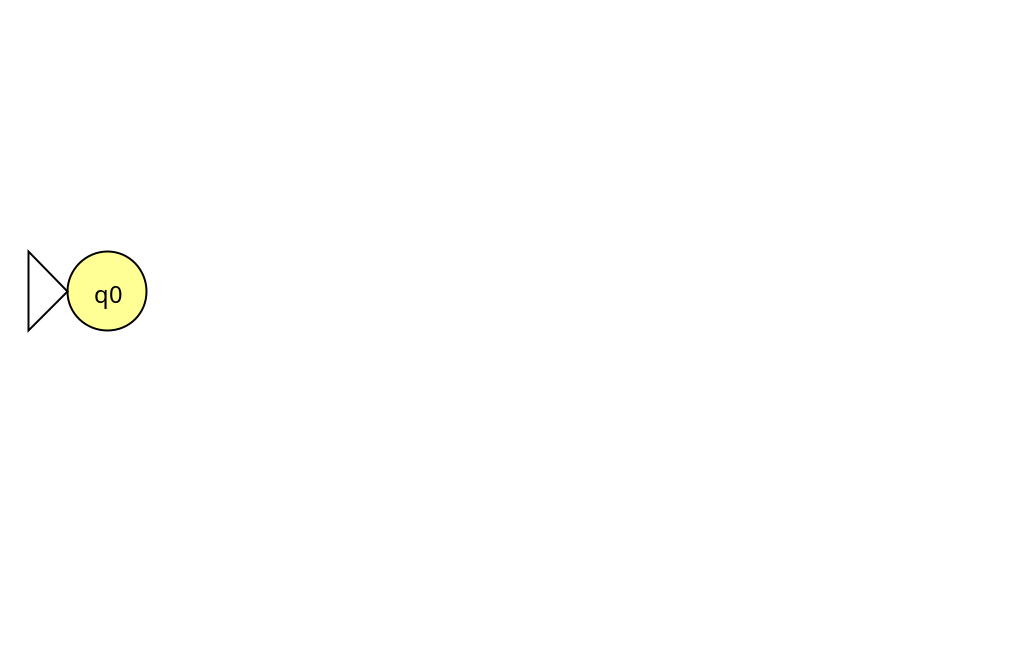
\includegraphics[scale=0.25]{images/mct1ej3_1.png}
    \end{figure}
\end{frame}

%%%%%%%%%%%%%%%%%%%%%%%%%%%%%%%%%%

\begin{frame}{Sección Cuarto de Punto}{Ejercicio 3}
    \textbf{Solución}\\
    \begin{figure}
        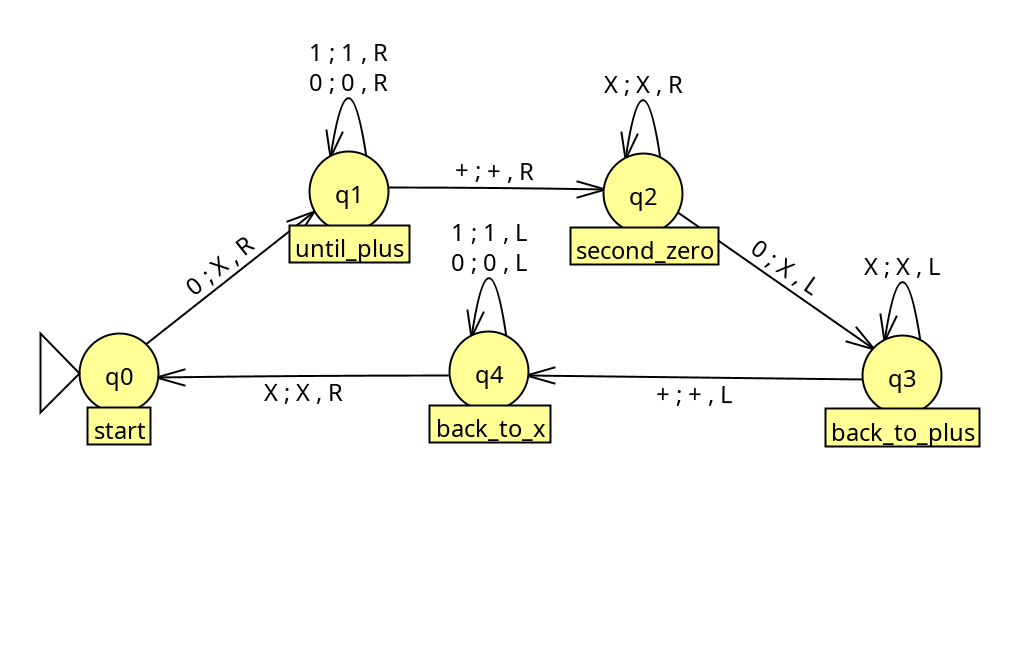
\includegraphics[scale=0.25]{images/mct1ej3_2.png}
    \end{figure}
\end{frame}

%%%%%%%%%%%%%%%%%%%%%%%%%%%%%%%%%%

\begin{frame}{Sección Cuarto de Punto}{Ejercicio 3}
    \textbf{Solución}\\
    \begin{figure}
        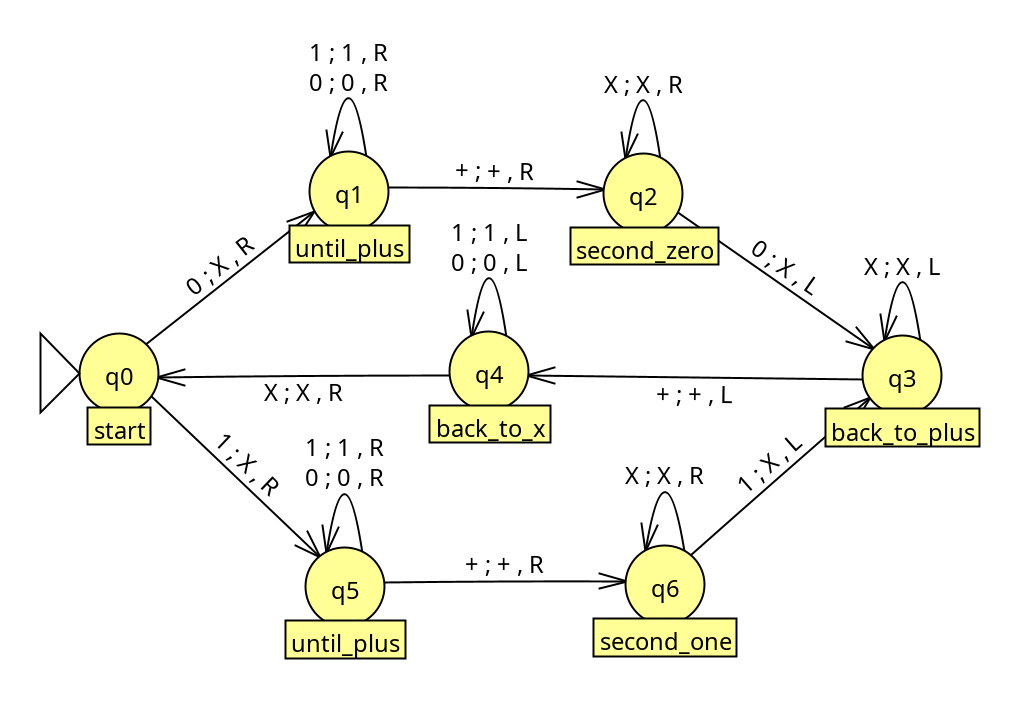
\includegraphics[scale=0.25]{images/mct1ej3_3.png}
    \end{figure}
\end{frame}

%%%%%%%%%%%%%%%%%%%%%%%%%%%%%%%%%%

\begin{frame}{Sección Cuarto de Punto}{Ejercicio 3}
    \textbf{Solución}\\
    \begin{figure}
        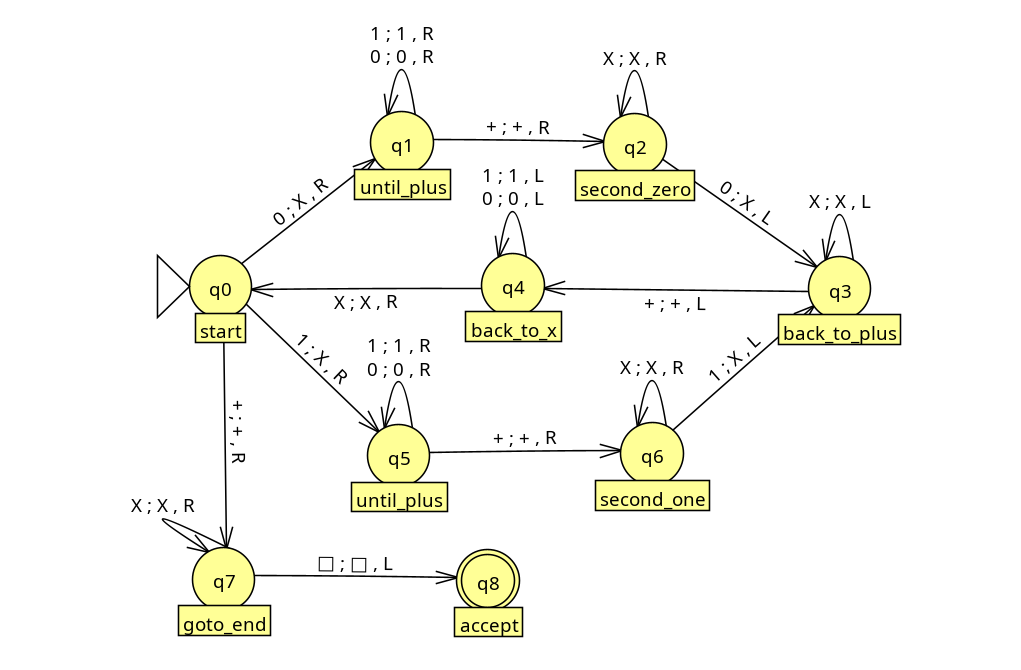
\includegraphics[scale=0.25]{images/mct1ej3_4.png}
    \end{figure}
\end{frame}

%%%%%%%%%%%%%%%%%%%%%%%%%%%%%%%%%%

\begin{frame}{Sección Cuarto de Punto}{Ejercicio 4}
% \vskip -1cm % Para subir (-) o bajar el texto
\textbf{Enunciado}
	\begin{itemize}
        \item Demostrar MT $\equiv$ SMT. Así, describe lo más formalmente posible el mecanismo para, a partir de un MT $M=(Q,\Sigma,\Gamma,\delta,q_0,q_f)$ conseguir la SMT equivalente $M'=(Q',\Sigma,\Gamma,\delta',q_0,q_f)$ y viceveresa.
	\end{itemize}
\end{frame}

%%%%%%%%%%%%%%%%%%%%%%%%%%%%%%%%%%

\begin{frame}{Sección Cuarto de Punto}{Ejercicio 4}
    \textbf{Solución}\\
    MT $\preceq$ SMT\\
    Trivial. Una MT $M=(Q,\Sigma,\Gamma,\delta,q_o,q_f)$ es una SMT sin transiciones con stay.
\end{frame}

%%%%%%%%%%%%%%%%%%%%%%%%%%%%%%%%%%

\begin{frame}{Sección Cuarto de Punto}{Ejercicio 4}
    \textbf{Solución}\\
    SMT $\preceq$ MT\\
    Sea $M=(Q,\Sigma,\Gamma,\delta,q_o,q_f)$ una SMT.\\ 
    Si $M$ no tiene ninguna transición con stay, entonces $M$ es una MT.\\
    Si no, para cada $q_i,q_j \in Q$ y $x,y \in \Gamma$ de forma que existe la transición $\delta(q_i,x)=(q_j,y,S)$ construimos un nuevo estado $q_{i,j,x,y}$.
    Sea $Q'$ el conjunto de estados formado por $Q$ y todos los $q_{i,j,x,y}$.
\end{frame}

%%%%%%%%%%%%%%%%%%%%%%%%%%%%%%%%%%

\begin{frame}{Sección Cuarto de Punto}{Ejercicio 4}
    \textbf{Solución}\\
    Entonces, sobre la quintupla $(Q',\Sigma,\Gamma,q_0,q_f)$ definimos la función $\delta':Q' \times \Gamma \rightarrow Q \times \Gamma \times \{L,R\}$ definida por:\\
    $\begin{cases}
        \delta'(q_i,x) = (q_j,y,L) & \text{si } \delta(q_i,x) = (q_j,y,L),\\
        \delta'(q_i,x) = (q_j,y,R) & \text{si } \delta(q_i,x) = (q_j,y,R),\\
        \delta'(q_i,x) = (q_{i,j,x,y},y,R) & \text{si } \delta(q_i,x) = (q_j,y,S),\\
        \delta'(q_{i,j,x,y},z) = (q_j,z,L) & \text{si } \delta(q_i,x) = (q_j,y,S) \text{ y } z \in \Gamma\\
    \end{cases}$
\end{frame}

%%%%%%%%%%%%%%%%%%%%%%%%%%%%%%%%%%

\begin{frame}{Sección Cuarto de Punto}{Ejercicio 4}
    \textbf{Solución}\\
    \begin{figure}
        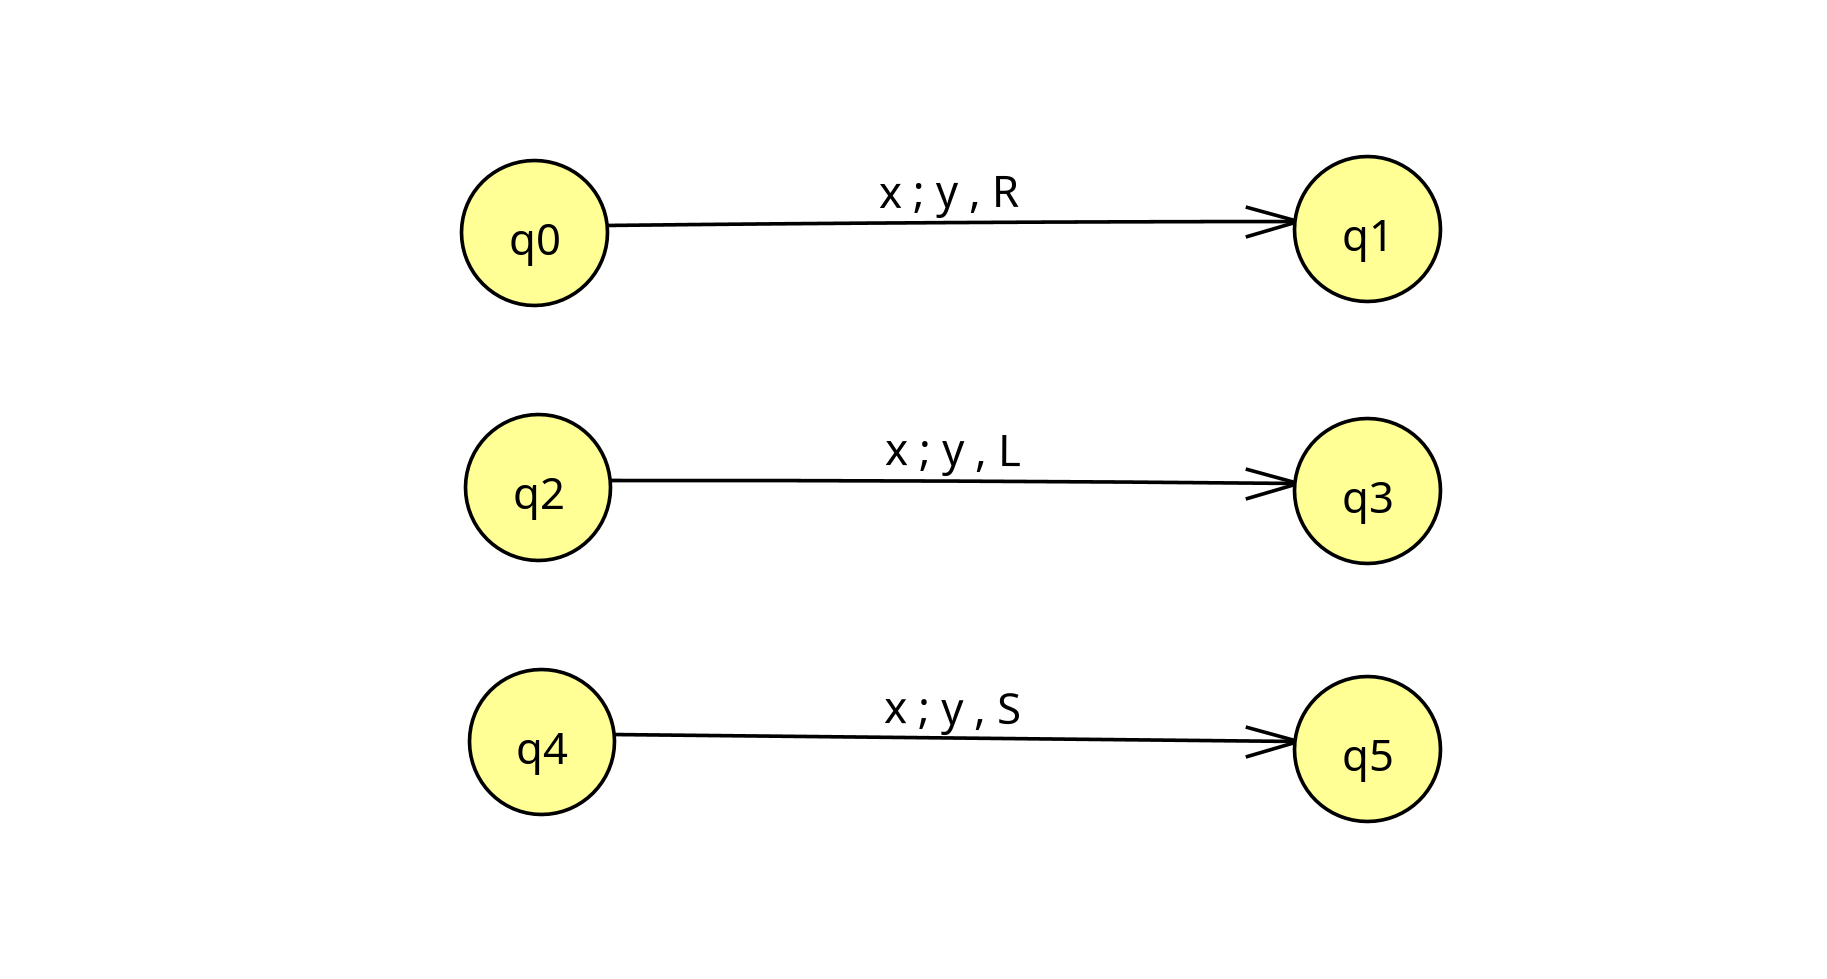
\includegraphics[scale=0.15]{images/mct1ej4_1.png}
    \end{figure}
\end{frame}

%%%%%%%%%%%%%%%%%%%%%%%%%%%%%%%%%%

\begin{frame}{Sección Cuarto de Punto}{Ejercicio 4}
    \textbf{Solución}\\
    \begin{figure}
        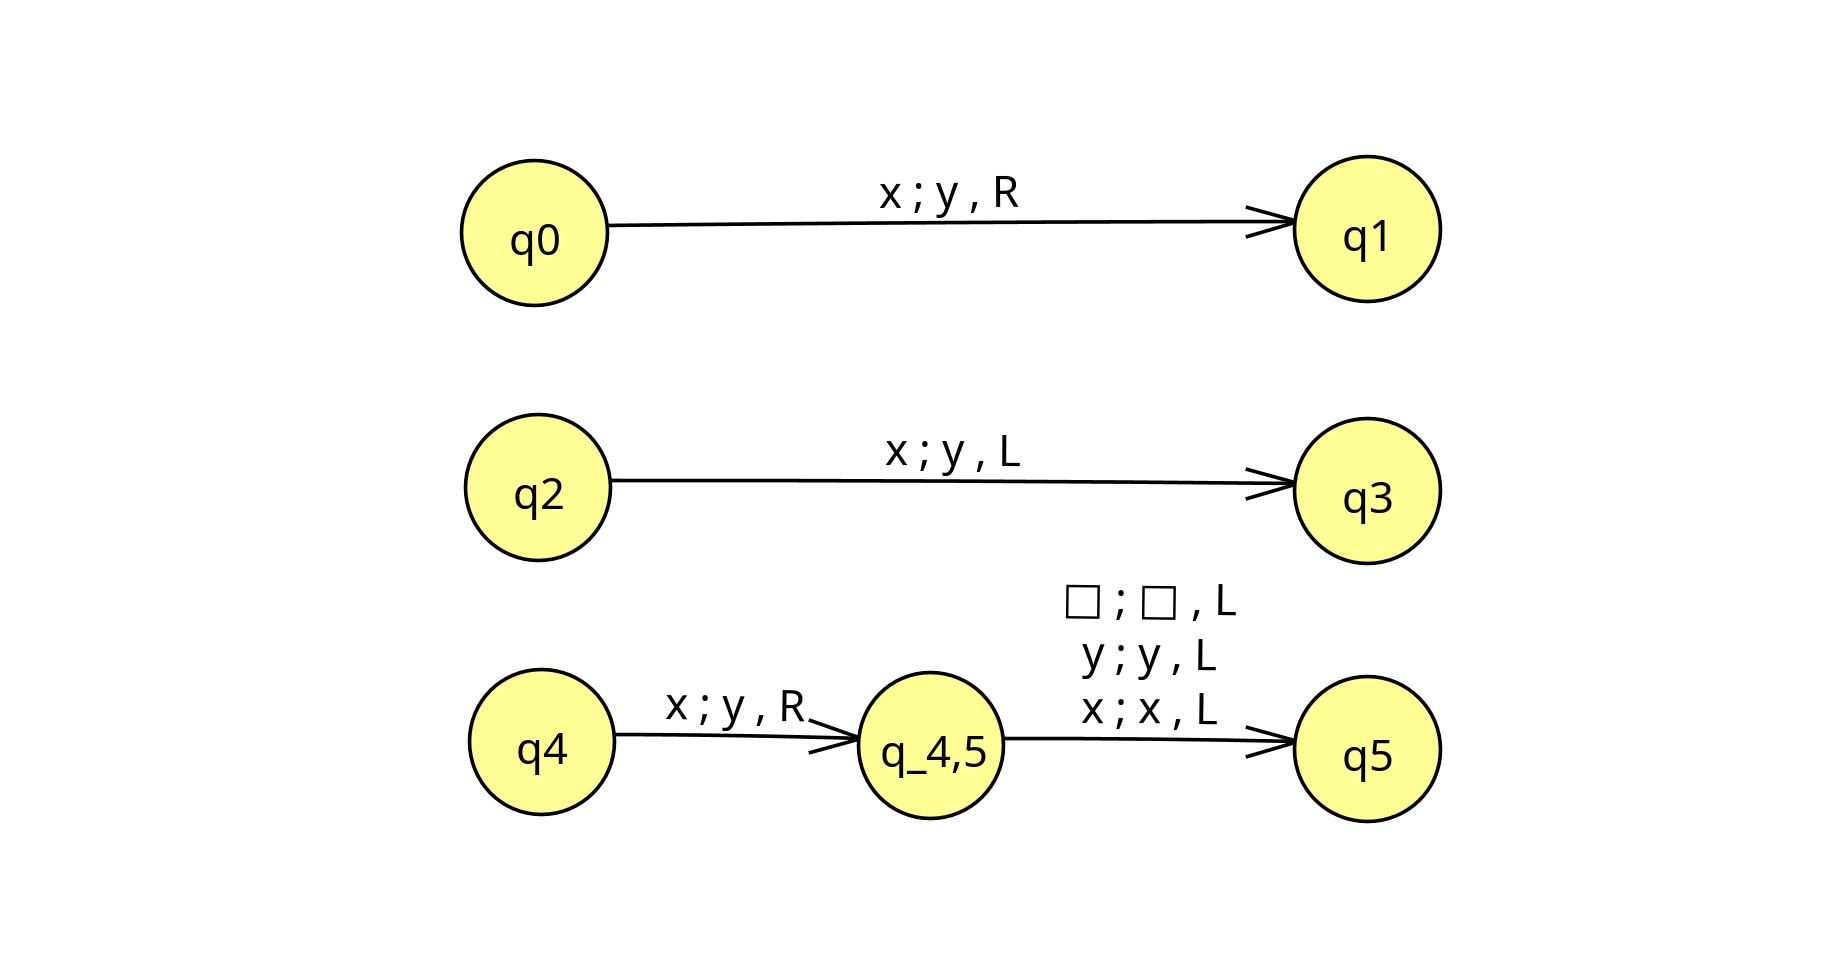
\includegraphics[scale=0.15]{images/mct1ej4_2.png}
    \end{figure}
\end{frame}


%%%%%%%%%%%%%%%%%%%%%%%%%%%%%%%%%%

\begin{frame}{Sección Cuarto de Punto}{Ejercicio 4}
    \textbf{Solución}\\
    \begin{figure}
        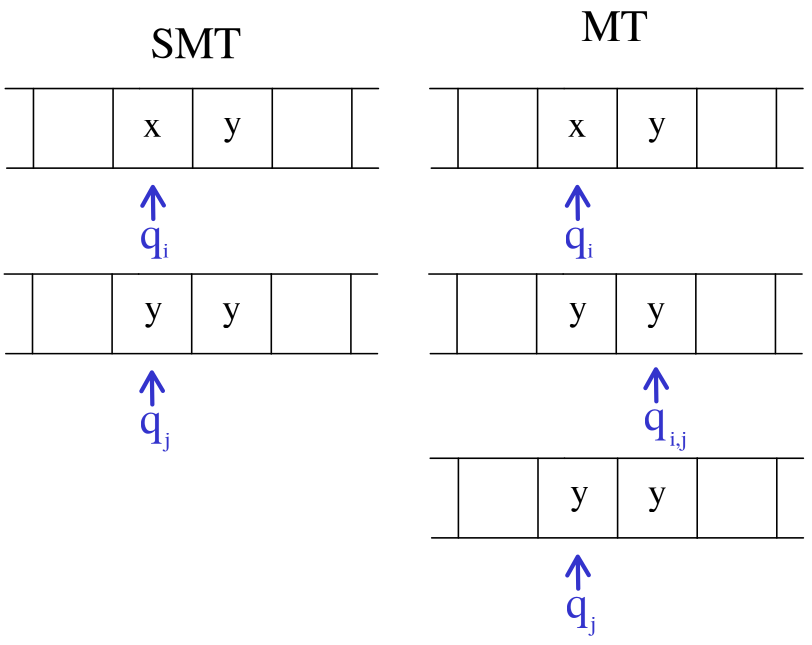
\includegraphics[scale=0.25]{images/mct1ej4_3.png}
    \end{figure}
\end{frame}

%%%%%%%%%%%%%%%%%%%%%%%%%%%%%%%%%%

\begin{frame}{Sección Cuarto de Punto}{Ejercicio 5}
% \vskip -1cm % Para subir (-) o bajar el texto
\textbf{Enunciado}
	\begin{itemize}
        \item Escribe en pseudocódigo una máquina de Turing para demostrar que el siguiente lenguaje es $\ld$. Acompaña la máquina con la explicación de los aspectos más relevantes. 
        \item[] $$HALT_{Q-steps}^{MT}=\{\langle M \rangle \mbox{ | M es MT y } \exists w \mbox{ con la que } M \mbox{ se detiene en }|Q| \mbox{ pasos o menos}  \}$$
    \end{itemize}
\end{frame}

%%%%%%%%%%%%%%%%%%%%%%%%%%%%%%%%%%

\begin{frame}{Sección Cuarto de Punto}{Ejercicio 5}
    \textbf{Solución}\\
    La solución es...
\end{frame}

%%%%%%%%%%%%%%%%%%%%%%%%%%%%%%%%%%

\begin{frame}{Sección Cuarto de Punto}{Ejercicio 6}
% \vskip -1cm % Para subir (-) o bajar el texto
\textbf{Enunciado}
	\begin{itemize}
        \item Escribe una máquina de Turing para demostrar que el siguiente lenguaje es $\lr$. Acompaña la máquina con la explicación de los aspectos más relevantes. 
        \item[] $$ACC_{Q}^{MT}=\{\langle M \rangle \mbox{ | M es una MT y } |L(M)| \geq |Q| \mbox{ siendo Q el conjunto de estados de M}\}$$
    \end{itemize}
\end{frame}

%%%%%%%%%%%%%%%%%%%%%%%%%%%%%%%%%%

\begin{frame}{Sección Cuarto de Punto}{Ejercicio 6}
    \textbf{Solución}\\
    La solución es...
\end{frame}

%%%%%%%%%%%%%%%%%%%%%%%%%%%%%%%%%%

\begin{frame}{Sección Cuarto de Punto}{Ejercicio 7}
% \vskip -1cm % Para subir (-) o bajar el texto
\textbf{Enunciado}
	\begin{itemize}
        \item Demuestra por contraejemplo que no todo subconjunto de un lenguaje regular es regular y que no toodo subconjunto de un lenguaje libre de contexto es libre de contexto.
    \end{itemize}
\end{frame}

%%%%%%%%%%%%%%%%%%%%%%%%%%%%%%%%%%

\begin{frame}{Sección Cuarto de Punto}{Ejercicio 7}
    \textbf{Solución}\\
    La solución es...
\end{frame}

%%%%%%%%%%%%%%%%%%%%%%%%%%%%%%%%%%

\begin{frame}{Sección Cuarto de Punto}{Ejercicio 8}
% \vskip -1cm % Para subir (-) o bajar el texto
    \textbf{Enunciado}
    \begin{itemize}
        \item El conjunto $\mt$ de las máquinas de Turing es numerable. La numeración de Gödel es prueba de ello. A partir del lenguaje simple que se ha dado en clase, calcula el número de Gödel de cada una de las instrucciones que componen este fragmento y del fragmento en si. ¿Es posible que dos fragmentos distintos tengan el mismo número?
        \begin{itemize}
            \item[] $V_1 \coloneqq S(0)$
            \item[] $V_2 \coloneqq S(V_1)$
            \item[] If $S(V_2)!=0$ Then $V_2 \coloneqq0$
            \item[] If $S(V_1)=0$ Then $V_1 \coloneqq S(V_2)$
            \item[] $V_1 \coloneqq S(S(V_2))$
        \end{itemize}
    \end{itemize}
\end{frame}

%%%%%%%%%%%%%%%%%%%%%%%%%%%%%%%%%%

\begin{frame}{Sección Cuarto de Punto}{Ejercicio 8}
    \textbf{Solución}\\
    La solución es...
\end{frame}

%%%%%%%%%%%%%%%%%%%%%%%%%%%%%%%%%%

\begin{frame}{Sección Cuarto de Punto}{Ejercicio 9}
% \vskip -1cm % Para subir (-) o bajar el texto
    \textbf{Enunciado}
    \begin{itemize}
        \item La Máquina de Turing Universal (también llamada $U$), como todas las MTs tiene un número de Gödel asociado. Aunque el número depende de la codificación elegida, investiga en Internet alguna versión del número de la MT Universal. ¿Cuántos  dígitos tiene? Explica cómo has llegado a la solución.
    \end{itemize}
\end{frame}

%%%%%%%%%%%%%%%%%%%%%%%%%%%%%%%%%%

\begin{frame}{Sección Cuarto de Punto}{Ejercicio 9}
    \textbf{Solución}\\
    La solución es...
\end{frame}

%%%%%%%%%%%%%%%%%%%%%%%%%%%%%%%%%%

\begin{frame}{Sección Cuarto de Punto}{Ejercicio 10}
% \vskip -1cm % Para subir (-) o bajar el texto
    \textbf{Enunciado}
    \begin{itemize}
        \item ¿Son decidibles los siguientes lenguajes? ¿Y Turing-reconocibles? Justifica tus respuestas:
        \begin{enumerate}[a)]
            \item  $\{\langle M \rangle \mbox{| M es MT y  M es la única MT que acepta } L(M)\}$ 
            \item $\{\langle M \rangle \mbox{| M es MT  y  se puede diseñar un programa en Java para reconocer } L(M)\}$
        \end{enumerate}
    \end{itemize}
\end{frame}

%%%%%%%%%%%%%%%%%%%%%%%%%%%%%%%%%%

\begin{frame}{Sección Cuarto de Punto}{Ejercicio 10}
    \textbf{Solución}\\
    La solución es...
\end{frame}

%%%%%%%%%%%%%%%%%%%%%%%%%%%%%%%%%%

\begin{frame}{Sección Medio Punto}{Ejercicio 11}
% \vskip -1cm % Para subir (-) o bajar el texto
    \textbf{Enunciado}
    \begin{itemize}
        \item Sea $\Sigma=\{0,1,\$\}$. Sea el lenguaje $L=\{x\$x^R\$x \mid x \in \Sigma^*\}$. Demostrar que no es regular: primero explica el lenguaje poniendo algunas palabras ejemplo, luego explica los conceptos teóricos que te van a servir en la demostración, el método de demostración que vas a usar y, finalmente la demostración en si.
    \end{itemize}
\end{frame}

%%%%%%%%%%%%%%%%%%%%%%%%%%%%%%%%%%

\begin{frame}{Sección Medio Punto}{Ejercicio 11}
    \textbf{Solución}\\
    La solución es...
\end{frame}

%%%%%%%%%%%%%%%%%%%%%%%%%%%%%%%%%%

\begin{frame}{Sección Medio Punto}{Ejercicio 12}
% \vskip -1cm % Para subir (-) o bajar el texto
    \textbf{Enunciado}
    \begin{itemize}
        \item Sea $L= \{ 0^i 1^j 2^k \mid i,j,k \geq0 \mbox{; si } i=1 \mbox{ entonces } j=k \} $. Este lenguaje no es regular. En este caso nos basta con que des una  demostración informal. Pero muestra que, sin embargo,  $L$ sí cumple el Lema del Bombeo para los Lenguajes Regulares.
    \end{itemize}
\end{frame}

%%%%%%%%%%%%%%%%%%%%%%%%%%%%%%%%%%

\begin{frame}{Sección Medio Punto}{Ejercicio 12}
    \textbf{Solución}\\
    La solución es...
\end{frame}

%%%%%%%%%%%%%%%%%%%%%%%%%%%%%%%%%%

\begin{frame}{Sección Medio Punto}{Ejercicio 13}
% \vskip -1cm % Para subir (-) o bajar el texto
    \textbf{Enunciado}
    \begin{itemize}
        \item Rellena cada casilla de la siguiente tabla con la clase más específica a la que pertenece el lenguaje  $\overline{L_1 \setminus L_2}$ siendo $L_1$ un lenguaje que cumple el supuesto expresado por su fila y $L_2$ siendo un lenguaje que cumple el supuesto dado por su columna. Si algún caso no se puede saber, puedes poner   $"?"$. Justifica cada casilla.\\
    \end{itemize}
\end{frame}

%%%%%%%%%%%%%%%%%%%%%%%%%%%%%%%%%%

\begin{frame}{Sección Medio Punto}{Ejercicio 13}
    \textbf{Solución}\\
    \begin{table}[h]
             \begin{tabular}{|l|l|l|l|}
             \hline
             &&&\\
             &$L_2 \in \lcf$ &$ L_2 \in \ld$ & $ L_2 \in \lr$\\
             \hline
             &&&\\
              $ L1 \in \lreg$&(1)&(2)&(3)\\
              \hline
             &&&\\
             $ L1 \subset L$, con $L \in \lcf$&(4)&(5)&(6)\\
              \hline
             &&&\\
             $L1 \in CO-\lr $&(7)&(8)&(9)\\
              \hline
             &&&\\
             $L1 \in \lr \cap CO-\lr$&(10)&(11)&(12)\\
              \hline
             &&&\\
             $ L1 \in \lr \setminus CO-\lr$&(13)&(14)&(15)\\
              \hline
             \end{tabular}
        \end{table}
\end{frame}

%%%%%%%%%%%%%%%%%%%%%%%%%%%%%%%%%%

\begin{frame}{Sección Medio Punto}{Ejercicio 14}
% \vskip -1cm % Para subir (-) o bajar el texto
    \textbf{Enunciado}
    \begin{itemize}
        \item Se tienen las hipótesis de A a E y se tienen las conclusiones de I a V. Se pide conectar cada hipótesis con las conclusiones que se pueden deducir de cada una (pueden ser varias) y dar una breve explicación.
    \end{itemize}
\end{frame}

%%%%%%%%%%%%%%%%%%%%%%%%%%%%%%%%%%

\begin{frame}{Sección Medio Punto}{Ejercicio 14}
% \vskip -1cm % Para subir (-) o bajar el texto
    \textbf{Hipótesis}
    \begin{enumerate}[A.]
        \item $\overline{L} \in CO-\lr$, $X$ es \lr-completo y $X \le_m  L$
        \item El cardinal de $L$ es un número natural
        \item $L \le_m  EQ^{DFA}$  
        \item $EQ^{MT} \le_m L$ 
        \item Existe una MT que acepta las cadenas que son de $L$ y una MT que acepta las cadenas que no son de $L$. 
    \end{enumerate}
\end{frame}

%%%%%%%%%%%%%%%%%%%%%%%%%%%%%%%%%%

\begin{frame}{Sección Medio Punto}{Ejercicio 14}
% \vskip -1cm % Para subir (-) o bajar el texto
    \textbf{Conclusiones}
    \begin{enumerate}[I.]
        \item $L$ es  decidible.
        \item $L$ cumple el Lema de Bombeo para los Lenguajes  libres de contexto.
        \item se puede construir una MT que rechace las cadenas que son de $L$ y que acepte las cadenas que no son de $L$.
        \item $L$ no es recursivamente enumerable.
        \item $L$ es \lr-completo. 
    \end{enumerate}
\end{frame}

%%%%%%%%%%%%%%%%%%%%%%%%%%%%%%%%%%

\begin{frame}{Sección Medio Punto}{Ejercicio 14}
    \textbf{Solución}\\
    La solución es...
\end{frame}

%%%%%%%%%%%%%%%%%%%%%%%%%%%%%%%%%%

\begin{frame}{Sección Medio Punto}{Ejercicio 15}
% \vskip -1cm % Para subir (-) o bajar el texto
    \textbf{Enunciado}
    \begin{itemize}
        \item Demuestra la indecibilidad de K y la indecibilidad del Problema de la Parada usando descripciones gráficas de las MTs.
    \end{itemize}
\end{frame}

%%%%%%%%%%%%%%%%%%%%%%%%%%%%%%%%%%

\begin{frame}{Sección Medio Punto}{Ejercicio 15}
    \textbf{Solución}\\
    La solución es...
\end{frame}

%%%%%%%%%%%%%%%%%%%%%%%%%%%%%%%%%%

\begin{frame}{Sección Tres Cuartos de Punto}{Ejercicio 16}
% \vskip -1cm % Para subir (-) o bajar el texto
    \textbf{Enunciado}
    \begin{itemize}
        \item Demuestra que la operación de clausura es cerrada en $\lr$. Puedes usar una MT de alto nivel, pero da una breve explicación y detalla los aspectos claves de su funcionamiento.
    \end{itemize}
\end{frame}

%%%%%%%%%%%%%%%%%%%%%%%%%%%%%%%%%%

\begin{frame}{Sección Tres Cuartos de Punto}{Ejercicio 16}
    \textbf{Solución}\\
    La solución es...
\end{frame}

%%%%%%%%%%%%%%%%%%%%%%%%%%%%%%%%%%

\begin{frame}{Sección Tres Cuartos de Punto}{Ejercicio 17}
% \vskip -1cm % Para subir (-) o bajar el texto
    \textbf{Enunciado}
    \begin{itemize}
        \item Justifica la verdad o falsedad de los siguientes enunciados:
        \begin{enumerate}[a)]
            \item Sea $L_2 \in \lr$ y sea $L_1$ tal que $L_1 \subseteq L_2$. Entonces, si $\exists$ un autómata con pila $A$ tal que $L(A)=L_2$ entonces $L_1$ cumple el Lema de Bombeo para los Lenguajes Libres de Contexto. 
            \item Sea $L_2 \in \lr$ y sea $L_1$ tal que $L_1 \subseteq L_2$. Entonces, si no  existe una máquina de Turing con  STAY para decidir $L_1$ entonces no existe una máquina de Turing determinista de 2 cintas para decidir $L_2$.
            \item Sea $L_2 \in \lr$ y sea $L_1$ tal que $L_1 \subseteq L_2$. Entonces, si $L_2 \setminus L_1=\{\lambda\}$ se cumple que si $L_1 \in \ld$ entonces $L_2 \in \ld$ .
            \item ...
        \end{enumerate}
    \end{itemize}
\end{frame}

%%%%%%%%%%%%%%%%%%%%%%%%%%%%%%%%%%

\begin{frame}{Sección Tres Cuartos de Punto}{Ejercicio 17}
    \textbf{a) Sea $L_2 \in \lr$ y sea $L_1$ tal que $L_1 \subseteq L_2$. Entonces, si $\exists$ un autómata con pila $A$ tal que $L(A)=L_2$ entonces $L_1$ cumple el Lema de Bombeo para los Lenguajes Libres de Contexto.}\\
    La solución es...
\end{frame}

%%%%%%%%%%%%%%%%%%%%%%%%%%%%%%%%%%

\begin{frame}{Sección Tres Cuartos de Punto}{Ejercicio 17}
    \textbf{b) Sea $L_2 \in \lr$ y sea $L_1$ tal que $L_1 \subseteq L_2$. Entonces, si no  existe una máquina de Turing con  STAY para decidir $L_1$ entonces no existe una máquina de Turing determinista de 2 cintas para decidir $L_2$.}\\
    La solución es...
\end{frame}

%%%%%%%%%%%%%%%%%%%%%%%%%%%%%%%%%%

\begin{frame}{Sección Tres Cuartos de Punto}{Ejercicio 17}
    \textbf{c) Sea $L_2 \in \lr$ y sea $L_1$ tal que $L_1 \subseteq L_2$. Entonces, si $L_2 \setminus L_1=\{\lambda\}$ se cumple que si $L_1 \in \ld$ entonces $L_2 \in \ld$.}\\
    La solución es...
\end{frame}

%%%%%%%%%%%%%%%%%%%%%%%%%%%%%%%%%%

\begin{frame}{Sección Tres Cuartos de Punto}{Ejercicio 17}
    \textbf{d) Si $HALT^{MT} \le_m L$ entonces existe una MT  que acepte las cadenas de $L$ y rechace las cadenas que no son de $L$.}\\
    La solución es...
\end{frame}

%%%%%%%%%%%%%%%%%%%%%%%%%%%%%%%%%%

\begin{frame}{Sección Tres Cuartos de Punto}{Ejercicio 17}
    \textbf{e) El lenguaje $L_{exquisito}$, formado por aquellas MTs que aceptan menos cadenas de las que no aceptan, es indecidible. (además, descríbelo como los lenguajes de clase).}\\
    La solución es...
\end{frame}

%%%%%%%%%%%%%%%%%%%%%%%%%%%%%%%%%%

\begin{frame}{Sección Tres Cuartos de Punto}{Ejercicio 17}
    \textbf{f) El lenguaje $$L_{not_{murciano}}=\{\langle M \rangle \mid \mbox{M es MT  tal que } |w|\neq |pijo|,  \forall w \in L(M) \}$$  no es decidible según el Teorema de Rice}\\
    La solución es...
\end{frame}

%%%%%%%%%%%%%%%%%%%%%%%%%%%%%%%%%%

\begin{frame}{Sección Tres Cuartos de Punto}{Ejercicio 17}
    \textbf{g) Si $L\le_m  Acc^{PDA}$ entonces existe una MT de 2 cintas que decide $L$. }\\
    La solución es...
\end{frame}

%%%%%%%%%%%%%%%%%%%%%%%%%%%%%%%%%%

\begin{frame}{Sección Tres Cuartos de Punto}{Ejercicio 17}
    \textbf{h) Dada  una propiedad trivial $PT$ de los lenguajes \lr y $L_{PT}=\{\langle M \rangle \mid \hbox{ M es una MT cuyo lenguaje no cumple } PT\}$, $L_{PT}$ es decidible y la MT que lo decide es una que siempre rechaza su entrada.}\\
    La solución es...
\end{frame}

%%%%%%%%%%%%%%%%%%%%%%%%%%%%%%%%%%

\begin{frame}{Sección Tres Cuartos de Punto}{Ejercicio 18}
% \vskip -1cm % Para subir (-) o bajar el texto
    \textbf{Enunciado}
    \begin{itemize}
        \item ¿Son decidibles los siguientes lenguajes? ¿Y Turing-reconocibles? Justifica tus respuestas:
        \begin{enumerate}[a)]
            \item $\{\langle M \rangle \hbox{| M es una MT con } |L(M)| \geq 100\}$ (por mapping-reducción desde $HALT^{MT}$)
            \item $\{\langle M \rangle \hbox{| M es una MT con lenguaje finito}  \}$ (por mapping-reducción desde $\overline{HALT^{MT}}$)
        \end{enumerate}
    \end{itemize}
\end{frame}

%%%%%%%%%%%%%%%%%%%%%%%%%%%%%%%%%%

\begin{frame}{Sección Tres Cuartos de Punto}{Ejercicio 18}
    \textbf{Solución}\\
    La solución es...
\end{frame}

%%%%%%%%%%%%%%%%%%%%%%%%%%%%%%%%%%

\begin{frame}{Sección Tres Cuartos de Punto}{Ejercicio 19}
% \vskip -1cm % Para subir (-) o bajar el texto
    \textbf{Enunciado}
    \begin{itemize}
        \item Sin usar el Teorema de Rice, demuestra la indecibilidad del lenguaje formado por MTs cuyos lenguajes son expresables por ERs.
    \end{itemize}
\end{frame}

%%%%%%%%%%%%%%%%%%%%%%%%%%%%%%%%%%

\begin{frame}{Sección Tres Cuartos de Punto}{Ejercicio 19}
    \textbf{Solución}\\
    La solución es...
\end{frame}

%%%%%%%%%%%%%%%%%%%%%%%%%%%%%%%%%%

\begin{frame}{Sección Dos Puntos}{Ejercicio 20}
% \vskip -1cm % Para subir (-) o bajar el texto
    \textbf{Enunciado}
    \begin{itemize}
        \item Demuestra la indecibilidad de los siguientes lenguajes sin usar el Teorema de Rice:
        \begin{enumerate}[a)]
            \item $\{\langle M \rangle \mid \mbox{M es MT y  se puede diseñar  un PDA A tal que L(A)=L(M)}\}$.
            \item Lenguaje formado por MTs  cuyos lenguajes son infinitos.
        \end{enumerate}
    \end{itemize}
\end{frame}

%%%%%%%%%%%%%%%%%%%%%%%%%%%%%%%%%%

\begin{frame}{Sección Dos Puntos}{Ejercicio 20}
    \textbf{Solución}\\
    La solución es...
\end{frame}


%%%%%%%%%%%%%%%%%%%%%%%%%%%%%%%%%%
%%%%%%%%%%%%%%%%%%%%%%%%%%%%%%%%%%
% BIBLIOGRAFÍA
%%%%%%%%%%%%%%%%%%%%%%%%%%%%%%%%%%
%%%%%%%%%%%%%%%%%%%%%%%%%%%%%%%%%%

% Redefinimos la apariencia
\setbeamertemplate{headline}{}
\setbeamertemplate{frametitle}{\vskip 0.5cm	\small{\textbf{\insertframetitle}}}
\setbeamertemplate{footline}{}

% Mostramos la bibliografía
% \begin{frame}[allowframebreaks] %% Si ocupa más de una página
\begin{frame} %% Si hay sólo una página
	\frametitle{Referencias}
	\footnotesize
	% \vskip -5cm %% Para ajustar la distancia al comienzo
	\bibliographystyle{abbrvnat}
	\bibliography{references}	
\end{frame}    
		
%%%%%%%%%%%%%%%%%%%%%%%%%%%%%%%%%%
%%%%%%%%%%%%%%%%%%%%%%%%%%%%%%%%%%

\end{document}

%%%%%%%%%%%%%%%%%%%%%%%%%%%%%%%%%%
%%%%%%%%%%%%%%%%%%%%%%%%%%%%%%%%%%